\documentclass[a4paper]{article}
\usepackage[utf8]{inputenc}
\usepackage{hyperref}
\usepackage[ngerman]{babel}
\usepackage{xcolor}
\usepackage{inconsolata}
\usepackage{listings}
\usepackage{caption}
\usepackage{etoolbox}
\usepackage{graphicx}
\usepackage{subfig}

\lstdefinestyle{c}{language=C,
basicstyle=\footnotesize\ttfamily,
commentstyle=\color{green},
identifierstyle=\color{blue},
keywordstyle=\color{purple},
stringstyle=\color{cyan},
numbers=left,
matchrangestart=t
}

% Needed so \autoref{fig:bla} writes Abbildung rather than Figure.
% From the Hyperref manual, p. 16/17, via https://tex.stackexchange.com/a/186948.
\addto\extrasngerman{%
  \def\figureautorefname{\figurename}%
}

% https://tex.stackexchange.com/a/110195
\makeatletter
\lst@Key{matchrangestart}{f}{\lstKV@SetIf{#1}\lst@ifmatchrangestart}
\def\lst@SkipToFirst{%
    \lst@ifmatchrangestart\c@lstnumber=\numexpr-1+\lst@firstline\fi
    \ifnum \lst@lineno<\lst@firstline
        \def\lst@next{\lst@BeginDropInput\lst@Pmode
        \lst@Let{13}\lst@MSkipToFirst
        \lst@Let{10}\lst@MSkipToFirst}%
        \expandafter\lst@next
    \else
        \expandafter\lst@BOLGobble
    \fi}
\makeatother

% http://www.latex-community.org/forum/viewtopic.php?f=4&t=2835
\definecolor{lightGray}{rgb}{0.9, 0.9, 0.9}
\newcommand{\Hilight}{\makebox[0pt][l]{\color{lightGray}\rule[-0.3em]{\linewidth}{1.2em}}}

\title{Stuxnet}
\author{Lucas Werkmeister}

\begin{document}

\maketitle

%\tableofcontents % should we have one?

\section{Einführung}

Stuxnet ist ein Computerwurm, der im Sommer 2010 entdeckt wurde.
Sein Ziel ist es, die iranische Urananreicherungsanlage in Natanz (und möglicherweise andere, etwa Buschehr) zu sabotieren.
Aufgrund seiner geschätzten Entwicklungszeit von 6 Monaten und 10 Entwicklern (plus Management, Testen, etc.),
die für einen Computerschädling enorm ist, sowie verschiedener anderer Faktoren
(etwa der Tatsache, dass zum Testen der Sabotage ein Nachbau einer Urananreicherungsanlage inklusive echtem Uran nötig gewesen sein muss),
wird geschätzt, dass der Urheber dieses Schädlings ein Staat sein muss;
als wahrscheinlichster Kandidat gelten die USA.
Mehrere Versionen (1.001, 1.100, 1.101) waren im Umlauf, die sich aber nur geringfügig unterscheiden.

2013 wurde eine Vorgängerversion von Stuxnet entdeckt, die die Versionsnummer 0.5 trägt.
Sie unterscheidet sich signifikant von Stuxnet 1.x und ist auch deutlich älter:
tatsächlich wurde Stuxnet 0.5 bereits 2007 auf der Antivirus-Plattform VirusTotal hochgeladen, aber nicht als Schädling erkannt.
Die Domains, zu denen Stuxnet 0.5 Kontakt aufnimmt (Command-and-Control), wurden sogar bereits 2005 registriert.

Wir werden im Folgenden bestimmte Komponenten von Stuxnet untersuchen und anschließend diese beiden Versionen vergleichen.

\section{Grundlagen der iranischen Urananreicherung}

\subsection{Urananreicherung}

Natürlich vorkommendes Uran besteht zu etwa 99\% aus dem Isotop $^{238}\mathrm U$ und zu etwa 1\% aus $^{235}\mathrm U$.
Nur letzteres Isotop ist zu einer Kernspaltungs-Kettenreaktion fähig.
Sein Anteil muss zur Energiegewinnung auf 3-5\%, für Nuklearwaffen sogar auf über 85\% erhöht werden.
Diese \emph{Anreicherung} des Urans geschieht üblicherweise durch Gaszentrifugen.
Dabei wird das Gas $\mathrm{UF}_6$, Uranhexafluorid, in einer Zentrifuge zur Rotation gebracht.
Fluor kommt als \emph{Reinelement} in der Natur ausschließlich als $^{19}F$ vor;
jegliche Gewichtsvariation unter den $\mathrm{UF}_6$-Molekülen ist also durch das enthaltene Uran verursacht.
In den Zentrifugen sammelt sich daher aufgrund der Zentrifugalkraft das $\mathrm{UF}_6$ mit dem erwünschten $^{235}\mathrm U$ innen,
während $\mathrm{UF}_6$ mit $^{238}\mathrm U$ außen entnommen werden kann.
Durch Wiederholung dieses Prozesses in einer Reihe von Zentrifugen wird das Uran angereichert.\cite{wiki:urananreicherung}

\subsection{Aufbau der Anlage im Iran}

Die Zentrifuge, die im Iran verwendet wird, ist das Modell \emph{IR-1}, ein europäisches Modell der späten sechziger Jahre.
Die Zentrifuge gilt als veraltet; ihr Hauptvorteil für Iran ist, dass sie massenhaft produziert werden kann.
Das ist wichtig, weil es Iran nie gelungen ist, die Zentrifuge zuverlässig zu betreiben:
obwohl die Ingenieure den Innendruck der Zentrifuge soweit gesenkt haben, dass sie nur noch die Hälfte ihrer theoretischen Maximalkapazität erreicht,
gehen die Zentrifugen regelmäßig kaputt.

Ein normaler Prozess zur Urananreicherung verträgt den Ausfall von Zentrifugen nur sehr schlecht.
Um dieses Problem zu umgehen, sind in den iranischen Anlagen Ventile an den Ein- und Ausgängen jeder Zentrifuge angebracht.
Fällt eine Zentrifuge aus, so kann sie durch die Ventile sofort vom restlichen Vorgang abgetrennt werden.
Da die Zentrifuge massenhaft produziert werden kann, steht Ersatz sofort zur Verfügung
(zu einem Zeitpunkt waren 4000 Zentrifugen im Einsatz und 5000 in Reserve\cite{tkac}), % p. 15
so dass die Zentrifuge direkt ausgetauscht werden kann.
Anschließend kann der Betrieb normal weiterlaufen.

\subsection{Steuerung der Anlage}

Die Urananreicherungsanlage wird durch sogenannte SCADA-Software kontrolliert.
Es ist unbekannt, welche Software genau im Iran zum Einsatz kommt;
nach einer Analyse von Langner\cite{tkac} handelt es sich aber um keines der üblichen Programme, % TODO exact cite
sondern um eine eigene Software.
Das Programm wird als amateurhaft eingestuft;
seine Autoren seien wohl mit modernem SCADA-Design wenig vertraut. % TODO ref

Das SCADA-Programm steuert allerdings nicht direkt die Zentrifugen;
es ist hauptsächlich ein Werkzeug zur Überwachung des Betriebs. % TKaC 9, Seite
Die direkte Steuerung der Zentrifugen geschieht stattdessen durch sog. Programmable Logic Controllers (PLCs).
Dabei handelt es sich um einfache Prozessoren, die Signale von Sensoren verarbeiten,
um Steuersignale zu setzen.
In der Anlage von Natanz stammt dieser Teil des Systems von Siemens;
der S7-315 Controller steuert die Rotoren der Zentrifugen selbst (164 Motoren pro Controller), % TKaC 12
der S7-417 Controller die Ventile, welche den Zu- und Abfluss von $\mathrm{UF}_6$ regeln (984 Zentrifugen pro Controller).
Diese PLCs werden durch die Siemens-Software \emph{Step7} (Eigenschreibweise \emph{STEP7}) programmiert;
indem Stuxnet dieses Programm infizierte, konnte es eigene Codeblöcke auf die PLCs schreiben
und somit den physikalischen Angriff durchführen.

\section{Physikalische Angriffe}

Stuxnet führte zwei Sabotage-Angriffe auf das Anreicherungssystem durch, die den Prozess stören sollten.
Der erste Angriff stammt aus Stuxnet 0.5.
In Stuxnet 1.x war er zwar noch enthalten, aber nicht mehr erreichbar (toter Code).
Dort kommt stattdessen ausschließlich der zweite Angriff zum Einsatz.
Da Stuxnet 0.5 noch nicht bekannt war, als Stuxnet 1.x untersucht wurde,
hielt man den ersten Angriff damals für ``Work in Progress''.\cite{dossier} % TODO exact ref
Hätten die Stuxnet-Autoren den ersten Angriff ganz aus Stuxnet 1.x entfernt,
so wäre die Verbindung zwischen den beiden Versionen vermutlich nie aufgefallen,
da sie ansonsten nur noch die Verbreitung über Step7 gemein haben.\cite{05} % TODO exact ref

\subsection{Erster Angriff: Ventile, Gasdruck (Stuxnet 0.5)}

Der erste Angriff manipuliert die Ventile an den Zentrifugen so,
dass $\mathrm{UF}_6$ zwar ein-, aber nicht mehr abfließen kann.
Dadurch steigt der Druck in den Zentrifugen.
Um dies vor den Operatoren der Anlage zu verbergen,
werden alte Sensordaten abgespielt, die Stuxnet vor Beginn des Angriffs aufzeichnet.

Würde Stuxnet nun nichts weiter tun, so würden die Zentrifugen durch den steigenden Druck schließlich zerstört werden.
Da aber ein Controller sehr viele Zentrifugen regelt (siehe open), würde dies für viele Zentrifugen fast zeitgleich geschehen;
dieses abnormale Verhalten würde auffallen und Stuxnet in einer Post-Mortem-Analyse vermutlich enttarnt werden.
Stuxnet bricht deshalb den Angriff nach einer Weile ab.
Dadurch verursacht dieser Angriff eine höhere Belastung der Anlage,
die durch eine höhere Ausfallrate der Zentrifugen langfristig den gleichen Schaden verursacht,
aber weniger auffällig ist und Stuxnet daher nicht enttarnt.

\subsection{Zweiter Angriff: Rotoren (Stuxnet 1.x)}

Der zweite Angriff manipuliert die Zentrifugen direkt, indem die Frequenz der Rotoren geändert wird.
Unter Normalbetrieb laufen die Rotoren auf 63000rpm (1050Hz).
Der Angriff läuft etwa monatlich und wechselt zwischen zwei Zuständen:
im ersten werden die Rotoren für 15 Minuten um gut ein Drittel auf 84600rpm (1410Hz) beschleunigt,
im zweiten werden über einen Zeitraum von 50 Minuten erst nahezu angehalten (120rpm, 2Hz) und dann wieder hochgefahren.
Die IR-1 läuft als \emph{superkritisches} Design im Normalbetrieb bereits über gewissen \emph{kritischen Geschwindigkeiten}
(entsprechend der Resonanzfrequenz des Systems), bei denen durch Resonanzen Vibrationen des Rotors auftreten können.
Wenn der Rotor nun im zweiten Zustand beinahe angehalten und wieder angefahren wird,
durchläuft er auch diese kritischen Frequenzen, mit dem Ergebnis einer noch höheren Ausfallwahrscheinlichkeit.

Stuxnet versucht ebenfalls, die Steuerungssoftware WinCC (falls in der Anlage vorhanden) zu verwenden, um den Angriff zwischen mehreren Controllern zu synchronisieren.\cite{dossier} % TODO exact cite
Dazu werden alle fünf Sekunden Pakete über das Netzwerk ausgetauscht; dieser Traffic sollte bei guter Aufsicht der Anlage nicht zu übersehen sein.
Dies, zusammen mit der Tatsache, dass die simultane Beschleunigung oder Abbremsung ganzer Reihen von Zentrifugen gut zu hören ist
(ein Controller steuert viele Zentrifugen, siehe oben) – noch verstärkt durch die Synchronisierung zwischen Controllern –
lässt vermuten, dass zur Entwicklung von Stuxnet 1.x weniger Wert darauf gelegt wurde, unentdeckt zu bleiben.

\section{Technische Wirkungsweise}

\subsection{Verbreitung von Stuxnet}

Auch bei der Verbreitung sind signifikante Unterschiede zwischen Stuxnet 0.5 und 1.x festzustellen:
Stuxnet 0.5 verbreitet sich ausschließlich über eine Sicherheitslücke in Step7.
Stuxnet 1.x hingegen weist zusätzlich dazu eine breite Vielfalt von Verbreitungswegen auf:

\begin{itemize}
\item Verbreitung über Memorysticks beim Ausführen von \texttt{autorun.inf}: nur Stuxnet 1.001\cite{dossier} % p. 30
\item Verbreitung über Memorysticks beim Betrachten von Ordnern mit bestimmten \texttt{.lnk}-Dateien (CVE-2010-2568\cite{CVE_lnk}): ab Stuxnet 1.100
\item Verbreitung über WinCC-Server (falls vorhanden) durch Ausnutzung eines hard-coded Server-Passworts (CVE-2010-2772\cite{CVE_wincc})
\item Verbreitung über das SMB-Netzwerkdateisystem
\item Verbreitung über Windows Server Service durch einen Fehler in RPC (Remote Procedure Call) (CVE-2008-4250\cite{CVE_rpc} / MS08-067\cite{MS_rpc})
\item Verbreitung über den Printer Spooler (CVE-2010-2729\cite{CVE_spooler} / MS10-061\cite{MS_spooler})
\end{itemize} % TODO welche davon sind zero-days?

\subsection{Updates erhalten}

Stuxnet verfügte auch einen Mechanismus, um sich selbst zu aktualisieren.
Updates wurden dabei von verschiedenen Servern heruntergeladen.

Für Stuxnet 0.5 wurde eine fiktive Werbeagentur ``MediaSuffix'' eingerichtet, die unter den folgenden Domains erreichbar war:

\begin{itemize}
\item \texttt{smartclick.org}
\item \texttt{best-advertising.net}
\item \texttt{internetadvertising4u.com}
\item \texttt{ad-marketing.net}
\end{itemize}

Die Server hinter den Domains standen in den Vereinigten Staaten, Kanada, Frankreich und Thailand; % 0.5 p. 4
die Domains sind heute alle entweder anderen Betreibern zugeordnet oder unerreichbar.

Normale Besucher sahen dort nur eine nichtssagende Hauptseite\cite{archive_best_advertising};
Stuxnet hingegen konnte auf einigen Unterseiten mit präparierten URLs eine Infektion zurückmelden oder Updates anfordern.

Für Stuxnet 1.x wurde eine neue Tarnung genutzt, offenbar für eine Sport\-wet\-ten-Agentur unter folgenden Domains:

\begin{itemize}
\item \texttt{mypremierfutbol.com}
\item \texttt{todaysfutbol.com}
\end{itemize}

Die Server hinter diesen Domains standen in Malaysia und Dänemark.
Un\-glück\-li\-cher\-wei\-se ist der damalige Inhalt dieser Seiten unbekannt,
da das Internet Archive sie erst seit 2011 archiviert,
nachdem sie bereits umgeleitet wurden, um weitere Stuxnet-Updates zu verhindern.

Auch Stuxnet 1.x rief präparierte URLs auf;
der Vorgang ist jedoch komplexer als bei Stuxnet 0.5.
Stuxnet sendet mehr Daten über das Hostsystem (zum Beispiel Betriebssystemversion, Hostname),
und die Kommunikation ist in beide Richtungen durch XOR-Verknüpfung mit statischen 31-Bit-Schlüsseln geschützt.

\subsection{Updates verteilen}

Da das schlussendliche Zielsystem von Stuxnet aus Sicherheitsgründen nicht direkt mit dem Internet verbunden ist,
müssen Updates über mehrere Stuxnet-Infektionen propagiert werden.

Stuxnet überprüft dazu vor jeder potenziellen Neuinfektion, ob das Zielsystem bereits infiziert ist;
ist dies der Fall, so werden die Versionen verglichen und gegebenenfalls das Zielsystem oder das eigene System aktualisiert.

Außerdem können Stuxnet-Infektionen auch direkt über das Netzwerk kommunizieren.
Stuxnet 0.5 verwendet dazu Mailslots, einen einfachen Mechanismus zur Interprozesskommunikation;
Stuxnet 1.x started hingegen einen vollständigen RPC-Server und -Client (RPC=Remote Procedure Call), % TODO proper abbreviations?
der verschiedene Programmroutinen bereitstellt und aufruft.

Ferner können File Shares, die wie oben erwähnt zur Infektion genutzt werden,
auch zur Kommunikation und zum Austausch von Stuxnet-DLLs dienen.

\subsection{CVE-2010-2743 Local Privilege Escalation (1.10x)}

Wir stelllen nun eine Sicherheitslücke in Windows vor, die Stuxnet ab Version 1.100 ausnutzte, um im Kernel-Mode zu laufen, genauer untersuchen.
Der Kern der Sicherheitslücke ist ein Zugriff durch Windows auf eine Funktionspointertabelle mit ungeprüftem Index.

Eine Funktionspointertabelle (Function Pointer Table) ist ein Mittel,
um effizient zwischen verschiedenen Verhaltensweisen eines Programms zu wählen.
In C kann sie so aussehen:

\lstinputlisting[
  language=C,
  style=c,
  caption=Implementierung und Verwendung einer Funktionspointertabelle,
  escapechar=\%
]{../functionPointerDemo2/01-harmless.c}

\texttt{execute()} führt eine unterschiedliche Operation aus, je nachdem, welche Funktion über das erste Argument ausgewählt wurde.
Anderer Code muss somit nur noch die Indizes (Opcodes) der einzelnen Operationen kennen, nicht mehr die Funktionen, die tatsächlich ausgeführt werden.

Allerdings ist das Verhalten von \texttt{execute()} undefiniert, wenn ein ungültiger Index eingegeben wird.
In diesem Fall wird Speicher gelesen, der nicht Teil der Funktionspointertabelle ist und vermutlich keinen gültigen Pointer in eine ausführbare Seite enthält;
das Ergebnis ist dann ein Segmentation Fault.

\lstinputlisting[
  language=C,
  style=c,
  firstline=19,
  caption=Ungültige Verwendung der \texttt{execute()}-Funktion,
  escapechar=\%
]{../functionPointerDemo2/02-broken.c}

Dies ist allerdings nicht zwingend gegeben; es ist durchaus möglich, dass an der richtigen Stelle ein Funktionspointer liegt,
etwa weil im Quelltext ein anderes Feld dahinter deklariert wurde, das ebenfalls einen Funktionspointer enthält:

\lstinputlisting[
  language=C,
  style=c,
  %linerange={7-7,14-14,20-25},
  caption=Ausführung von unbeabsichtigtem Code,
  escapechar=\%
]{../functionPointerDemo2/03-infected.c}

Im Falle von CVE-2010-2743 findet der Sprung in die Funktionspointertabelle innerhalb von \texttt{win32k.sys} beim Laden einer Tastaturbelegung statt.
Hinter der Funktionstabelle liegen hier nicht weitere Funktionspointer, sondern andere Daten.
Stuxnet lädt nun diese Systemdatei und durchsucht diese Daten nach einem geeigneten \texttt{DWORD}, das auch als virtuelle Adresse interpretiert werden kann.
Stuxnet könnte dort nun seinen eigenen Code hinschreiben. Allerdings ist der Platz an der Stelle möglicherweise begrenzt.
Stuxnet allokiert deshalb stattdessen freien Speicher und schreibt seinen Code dorthin.
An die Zieladresse des gefundenen \texttt{DWORD} wird dann nur ein Sprungbefehl an diese Stelle geschrieben.
Anschließend schreibt Stuxnet eine speziell korrupte Tastaturbelegungsdatei auf die Festplatte, die einen Sprung an das gefundene \texttt{DWORD} auslösen wird,
und weist dann Windows an, diese Tastaturbelegung zu laden.
Sobald \texttt{win32k.sys} (im Kernel-Mode laufend) versucht, in die Funktionstabelle zu springen,
läuft der eingeschleuste Stuxnet-Code ebenfalls im Kernel-Mode.

Der Fehler lässt sich sehr einfach beheben, indem der Index in die Funktionspointertabelle vor dem Sprung überprüft wird:

\lstinputlisting[
  language=C,
  style=c,
  linerange=19-26,
  caption=Fehlerbehandlung,
  escapechar=\%
]{../functionPointerDemo2/04-protected.c}

\subsection{CVE-2012-3015 Step7-Infektion}

Stuxnet infizierte auch Step7 und verbreitete sich über Step7-Projekte,
die zum Beispiel innerhalb der Anlage über USB-Sticks ausgetauscht wurden
(Stuxnet 0.5 verbreitete sich sogar \emph{ausschließlich} auf diesem Weg).
Außerdem wurde Step7 zur Infektion der PLCs genutzt, die dann letztlich den tatsächlichen, physikalischen Angriff durchführten.

Um eine Step7-Installation beim Öffnen eines Projekts zu infizieren, nutzt Stuxnet eine Untrusted Search Path Vulnerability (CWE-426\cite{cwe_searchpath}).
Durch eine manipulierte Konfigurationsdatei im Projekt wird Step7 veranlasst, eine bestimmte DLL-Datei zu laden.
Dabei sucht Step7 zwar erst auf dem System selbst (in der Step7-Installation sowie in verschiedenen Windows-Ordnern), % dossier p. 33
aber wenn die Datei dort nicht gefunden wird, sucht Step7 auch innerhalb des Pro\-jekt\-ord\-ners.
Dabei wird dann eine DLL gefunden, die von Stuxnet zuvor abgelegt wurde;
diese entschlüsselt und lädt wiederum eine andere Datei innerhalb des Projekts, welche den Haupt-Stuxnet-Code enthält.
Stuxnet läuft nun auf dem System und führt die restliche Infektion (Privilege Escalation, Infektion anderer Prozesse) durch.

Sobald Stuxnet auf dem System läuft, werden auch zwei Step7-DLLs mit eigenen Versionen ersetzt.
Die Stuxnet-Variante deklariert die gleichen Funktionen wie die Original-DLLs,
und die meisten der Funktionen leiten beim Aufruf auch nur an die Original-DLLs weiter,
welche umbenannt zu diesem Zweck weiterhin zur Verfügung stehen.
Einige Funktionen jedoch werden modifiziert, um die PLCs zu infizieren:
Dabei handelt es sich um Funktionen, die PLC-Blöcke schreiben, lesen und auflisten.
Indem Stuxnet diese Funktionen abfängt, kann es nicht nur eigenen Code auf die PLCs schreiben,
sondern auch verhindern, dass dieser Code entdeckt wird, indem er beim Lesen wieder herausgefiltert wird.
In anderen Worten, von einem infizierten System aus ist die Infektion der PLCs nicht zu erkennen.

% TODO erwähnen, wie spät gefixt? dass deshalb informationslage schlecht?

\section{Vergleich der Stuxnet-Versionen}

Wir vergleichen nun die Stuxnet-Versionen 0.5 und 1.x hinsichtlich ihrer Aggressivität und Verbreitungsweisen.

Stuxnet 0.5 verbreitet sich, wie schon erwähnt, ausschließlich über Step7-Infektionen.
Die Command-and-Control-Möglichkeiten sind darauf beschränkt, neuen Code herunterzuladen und auszuführen;
dies ist zwar ausreichend, um später eine neue Version mit weiterreichenden C\&C-Möglichkeiten (zum Beispiel Rück\-mel\-dung des Hostsystems) zu installieren,
zeigt aber, dass solche Fähigkeiten bei der Entwicklung von Stuxnet für unwichtig erachtet wurden.
Eine Verbreitung von Updates über das Netzwerk, um auch Computer zu erreichen, die keinen direkten Zugang zum Internet haben,
findet zwar statt, ist aber ebenfalls einfach gehalten.
Der tatsächliche Angriff auf die Zentrifugen ist hingegen sehr fortgeschritten:
er tarnt sich durch Abspielen von alten Sensordaten,
ist sehr präzise auf das Layout der Anlage zugeschnitten, so dass jegliche Änderung – unterschiedliche Zentrifugenanzahl, andere Anordnung der Stufen – ein Versagen des Angriffs zur Folge gehabt hätte,
und achtet sorgfältig darauf, unauffällig zu bleiben, indem der Angriff unterbrochen wird, bevor zu viele Zentrifugen auf einmal zerstört werden.
Es ist offensichtlich, dass bei Stuxnet 0.5 der Hauptentwicklungsaufwand auf diesen Angriff verwendet wurde,
während man für die Verbreitung keinen höheren Aufwand als nötig betrieb.

\begin{figure}
  \centering
  \subfloat[Ausgenutzte Sicherheitslücken]{
    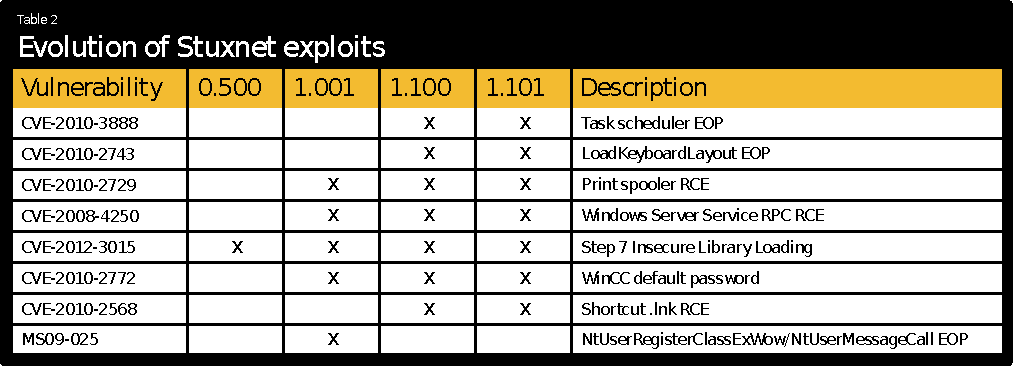
\includegraphics[width=0.75\linewidth]{../Evolution_exploits.pdf}
  }
  
  \subfloat[Verbreitungswege]{
    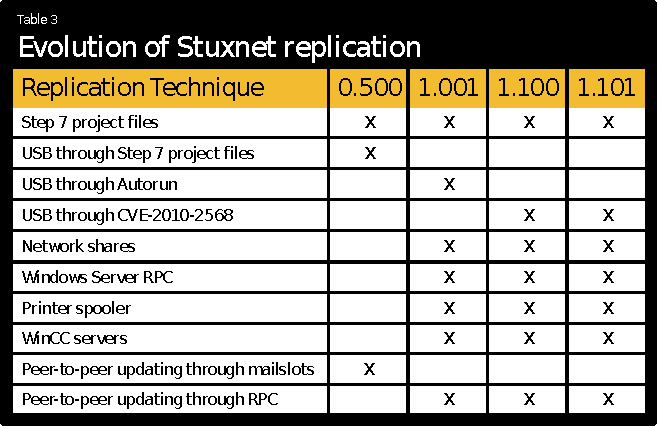
\includegraphics[width=0.5\linewidth]{../Evolution_replication.pdf}
  }
  \caption{Vergleich der Fähigkeiten der verschiedenen Stuxnet-Versionen\label{fig:vergleich}}
\end{figure}

Vollkommen anders ist die Situation bei Stuxnet 1.x.
Die Infektion von Step7 wurde unverändert übernommen (zur Laufzeit werden allerdings durch die Stuxnet-DLL mehr Funktionen abgefangen),
aber eine Vielzahl an Infektionswegen kam hinzu, einschließlich mehrerer Privilege Escalations, die dadurch nötig wurden (siehe \autoref{fig:vergleich}).
Stuxnet 1.x nutzt \emph{vier} Zero-Day-Exploits aus, eine enorm hohe Anzahl, die nie zuvor in Schädlingen nachgewiesen wurde
(die meiste Malware nutzt bekannte Sicherheitslücken; selbst ein Zero-Day-Exploit ist bereits selten).
Die Command-and-Control-Fähigkeiten sind ebenfalls weiter fortgeschritten;
Stuxnet lädt nicht nur neuen Code herunter (der, je nach Angabe des Servers, entweder im aktuellen oder per RPC in einem anderen Prozess ausgeführt wird),
sondern meldet zuvor auch verschiedene Informationen über sein Hostsystem,
inklusive Betriebssystem, Host- und Domainnamen, und ob Step7 oder WinCC vorhanden sind (Existenz bestimmter Registry-Keys).
Auch die Kommunikation unter Stuxnet-Infektionen ist ausgereifter:
anstelle einfacher Mailslots wird ein RPC-Server aufgesetzt, der zehn verschiedene Routinen bereitstellt. % dossier p. 25

Die Ausführung des tatsächlichen Angriffs steht in starkem Kontrast dazu:
der Angriff, der jetzt verwendet wird (Manipulation der Rotorgeschwindigkeit),
ist viel einfacher gehalten (der Angriff aus Stuxnet 0.5 ist weiterhin vorhanden, aber unerreichbar, und wurde zum Zeitpunkt der Untersuchung von Stuxnet 1.x für unfertig gehalten\cite{dossier}).
Dies hat den Vorteil, dass der Angriff relativ robust gegen Änderungen an der Anlage ist, die den 0.5-Angriff außer Gefecht gesetzt hätten.
Allerdings ist der Angriff auch leichter zu bemerken:
Ein Ingenieur, der sich ohne Gehörschutz in der Anlage befindet, würde die Beschleunigung und Bremsung der Zentrifugen leicht hören.
Dies wird dadurch noch verstärkt, dass Stuxnet versucht, den Angriff über mehrere PLCs hinweg zu synchronisieren
(falls ein infiziertes WinCC vorhanden ist);
diese Synchronisierung resultiert außerdem in Netzwerk-Traffic – alle 5 Sekunden – der den Aufsehern der Anlage hätte auffallen müssen.

Es ist also offensichtlich, dass sich zwischen Stuxnet 0.5 und 1.x der Fokus der Entwicklung
von der physikalischen Sabotage der Anlage zur Infektion ihrer Systeme verschob;
gleichzeitig wurde ein geringerer Wert darauf gelegt, nicht entdeckt zu werden.
Es wird spekuliert, dass eine Enthüllung von Stuxnet nicht nur in Kauf genommen wurde,
sondern sogar in einem gewissen Maße beabsichtigt war:
Stuxnet demonstriert deutlich, dass Cyber-Kriegsführung möglich und erfolgreich ist,
und es mag im Interesse der Stuxnet-Entwickler (mutmaßlich der USA) gewesen sein,
dass diese erste öffentliche Demonstration nicht von einem anderen Staat kam
(vergleichbar zum Space Race der USA mit der Sowjetunion,
wo letztere den USA mit Juri Gagarin als erstem Menschen im All zuvorkamen). % TKaC 16

\bibliographystyle{plain}
\bibliography{document}
\end{document}
